% Chapter Template

\chapter{A Benchmark for MTC Filesystems} % Main chapter title

\label{Chapter3} % Change X to a consecutive number; for referencing this chapter elsewhere, use \ref{ChapterX}

\lhead{Chapter 3. \emph{A Benchmark for MTC Filesystems}} % Change X to a consecutive number; this is for the header on each page - perhaps a shortened title

In the previous two chapters we have discussed about Many-Task Computing, how it is relevant for today's  computations and why it needs special filesystems. We looked at how those filesystems differ from regular disk-based ones, as well as why they need to be benchmarked differently. We also outlined the shortcomings of current benchmarks and how they can be surpassed. In this chapter, we focus on our approach to building an MTC-specific filesystem benchmark, the architecture behind it and the ways in which it can be used.

\section{Running coordinated commands across multiple nodes}\label{sec:coordination}

As we previously explained, in order to correctly benchmark access patterns on distributed filesystems, all nodes have to start running any given operation simultaneously. To solve this, we need to have a way of synchronizing nodes. Fortunately, synchronization is a common problem with multiple solutions in distributed programming frameworks.

To solve this problem, we used OpenMPI\cite{openmpi} barriers. We developed an MPI application that executes any given command on a set of available nodes. To do so, we spawn MPI workers in the default shared MPI communicator, we then synchronize them with the use of a barrier, and then the workers run the given command. By using the barrier, we can be sure that the command is run in a coordinated manner, at the same time.


\begin{figure}[H]
  \centering
    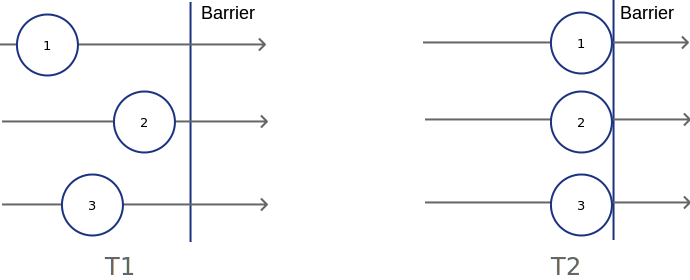
\includegraphics[scale=0.5]{Figures/barrier.png}
    \rule{25em}{0.5pt}
  \caption[MPI barrier]{Synchronizing processes with a barrier}
  \label{fig:barrier}
\end{figure}


% ---------------


\section{Why OpenMPI}

For our solution, we chose to use the MPI framework and, specifically, the OpenMPI\cite{openmpi} implementation. In this subsection we argument why.

Message Passing Interface (MPI) is a standardized communication protocol that is used to implement parallel computations. It defines an API that supports both collective (broadcast, scatter, gather) and point-to-point (send, receive) operations. Our solution makes use of both types of operations. We use a barrier to synchronize the nodes before running the core of the benchmark, and then we use point-to-point operations to send back the output from individual nodes to the master node, which aggregates the results. From our point of view, using MPI has two big advantages.

First, there are implementations available for most of the existing computer architectures existent today\cite{mpi_implementations}. This means that by using standard POSIX and MPI in a program, it can run with no extra porting work on multiple architectures. Since we want our benchmark to be accessible to everybody, portability is a great concern. To achieve this, we made sure to only use standard APIs and to not rely on any implementation-specific behavior in our code.

Second, MPI is built to scale natively. This means that we can write the code for a distributed application once and then run it on any number of nodes without having to change anything. The way this works at the API level is fairly simple - all instances are together in a container (called communicator) and within that container they all have a rank (which is an integer identifier).


Because MPI was implemented for a multitude of different architectures, it is generally supported on computer clusters. We developed our solution on the DAS4\cite{das4} cluster which has support for multiple MPI implementations:

\begin{itemize}

\item OpenMPI
\item MPICH
\item MPICH2
\item Intel MPI

We decided to use OpenMPI mainly because of its open source and vendor-independent nature. However, if OpenMPI is not available for some users of our benchmark, they can use any other implementation without problems, as our code relies only on standard behavior.

\end{itemize}

% ----------

\section{Aggregating the outputs of multiple nodes}

Having an MPI program that runs any given command across multiple nodes, we need a way to capture the outputs and then aggregate them. This is needed because benchmarks like IOzone and mdtest display the performance statistics on the standard output (stdout). Our distributed program has every slave node capture its own output then send it back to the master node, which in turn aggregates all outputs and formats them accordingly.

\begin{figure}[H]
  \centering
    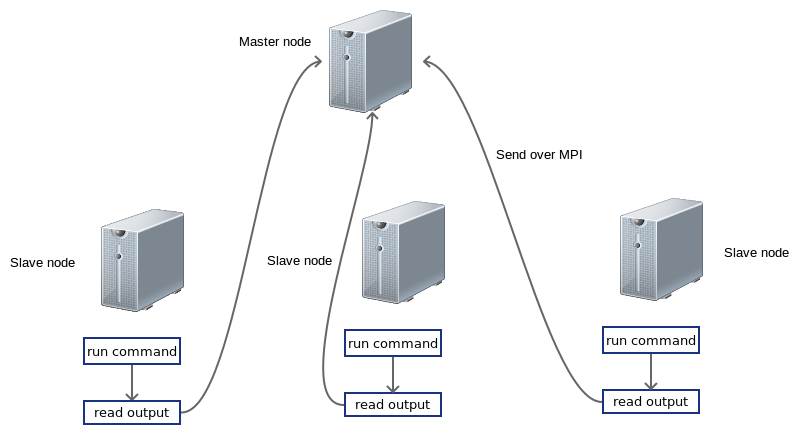
\includegraphics[scale=0.5]{Figures/slave_send_output.png}
    \rule{25em}{0.5pt}
  \caption[Slave nodes sending output]{Slave nodes sending output to master node}
  \label{fig:slave_send_output}
\end{figure}


To solve this problem, our initial solution was to use the \textit{popen}\cite{popen} system call. This runs a given command and captures its output. Then, that output can be sent over MPI to the master node for aggregation. While this approach worked when testing locally using threads, when we tested across distributed nodes using the network stack for communication, the process failed. We discovered that this is due to the fact that \textit{popen} uses \textit{fork} and pipes, which MPI does not fully support.

Since using \textit{popen} was not possible, we found that we could run commands with \textit{system}\cite{system}. However, \textit{system} does not provide a way to capture output, so we had to overcome this new limitation. We did so by making use of output redirection. This means that when we call an external command, we redirect its output to a temporary file that is local to the node, read the output from there and then delete that file.

\begin{figure}[H]
  \centering
    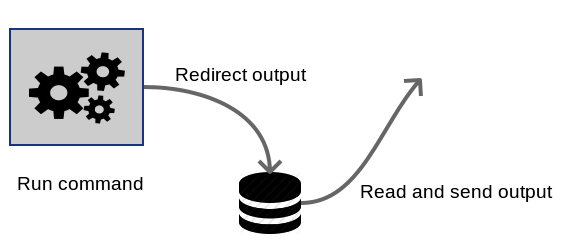
\includegraphics[scale=0.5]{Figures/local_exec.png}
    \rule{25em}{0.5pt}
  \caption[Local command execution]{Local execution on the slave node}
  \label{fig:local_exec}
\end{figure}


% --------------

\section{Varying the number of nodes}

An important aspect of distributed software of any kind is scalability - what is the relation between performance and number of nodes? Naturally, this is relevant for MTC filesystems as well. To measure this, we need to run the same benchmark on different numbers of nodes and then compare the results.

Since this is a given in MTC filesystem benchmarking, our solution handles this by default. The user can configure on what series of node numbers they want the test to run, and the benchmark will measure scalability automatically. To achieve this, we re-run the benchmark with more and more of the available nodes and keep track of the results.

\begin{figure}[H]
  \centering
    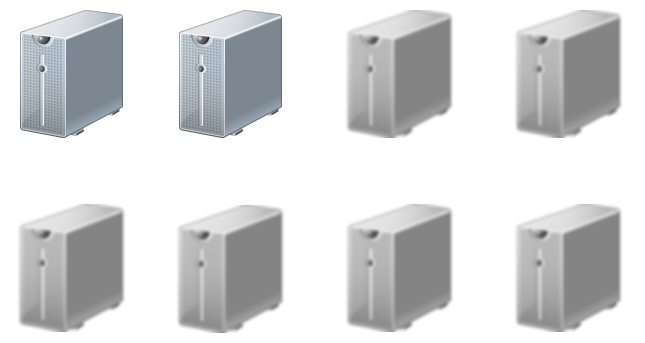
\includegraphics[scale=0.5]{Figures/nodes_grayed.png}
    \rule{25em}{0.5pt}
  \caption[Varying the number of nodes]{Varying the number of nodes}
  \label{fig:nodes_grayed}
\end{figure}

The implementation consists of a Python wrapper over the MPI code mentioned in Section~\ref{sec:coordination}. It iterates over an array of integers representing node counts and runs the benchmark with the given amount of nodes. Because it uses the MPI code, it needs to tell MPI exactly what nodes to use. This is done using a machinefile - a text file that contains node IPs, one per line. The MPI program always uses the same machinefile, and the Python wrapper updates it between runs as necessary, increasing the number of nodes.

Because clusters usually have a reservation process that a user has to go through before having access to a set of nodes, we added support for that to our solution as well. For this, we provide a \textit{reserve.sh} script that takes a number of nodes as argument and reserves that many nodes on the cluster. It also checks if the user already has reserved nodes and if so, it reuses those. The Python wrapper uses this script to reserve the maximum amount of nodes needed at the beginning of the run, and then uses them increasingly as the tests advance. So, if the user specified the array \textit{[1, 2, 4, 8, 16]} for the amounts of test nodes, the benchmark would reserve 16 nodes from the start and then run the tests with 1, 2, 4 (and so on) nodes.

The reason for which we kept the node reservation process in a separate script is that other clusters might require different commands to reserve nodes. We want our solution to be accessible to as many users as possible, and running on a different cluster shouldn't imply changing the benchmark's code. This way, the only necessary change is to adapt the \textit{reserve.sh} script.

In order to properly support multiple nodes in tests, there also needs to be a way to parametrize the given commands by nodes. For example, maybe the user wants node 3 to run IOzone against \texttt{test\_file\_3}. To achieve this, our tool sets an environment variable to the ID of every node, such that examining \texttt{\$\{NODENAME\}} on node 3 will yield \texttt{3}.

% ----------

\section{Leveraging existing benchmarks}

As discussed in Chapter~\ref{Chapter2}, our solution builds on top of existing benchmarks, adding only what is lacking in order to provide a complete MTC filesystem benchmark. Thus, we can decompose it into 5 distinct components:

\begin{itemize}

\item IOzone (3rd party benchmark)
\item mdtest (3rd party benchmark)
\item the MPI coordination program
\item a set of parsers for IOzone and mdtest ouputs
\item a set of plotters for IOzone and mdtest results

\end{itemize}

\begin{figure}[H]
  \centering
    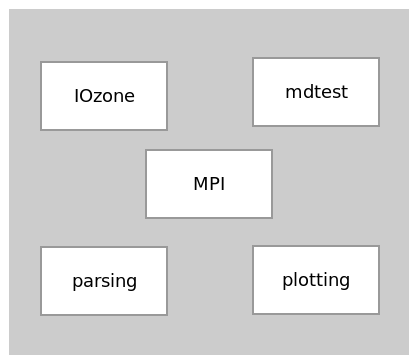
\includegraphics[scale=0.5]{Figures/components.png}
    \rule{25em}{0.5pt}
  \caption[Components]{Components}
  \label{fig:components}
\end{figure}

Having already discussed about IOzone and mdtest in Chapter~\ref{Chapter2}, this section explains how our solution makes use of them, as well as how it processes their results, from unstructured blobs of output to structured data, and then to plots.


\subsection{IOzone}

IOzone's main use is for measuring performance on reads and writes. Our project uses it for the read and write throughput measuring that is specified by the MTC Envelope.

For the 1-to-1 test cases, we let IOzone create the test files. However, for the N-to-1 test cases, we create a file using \textit{dd} before running IOzone, and then (for N-to-1 reads) we have all IOzone processes test the read/re-read performance on that particular file.

Out of the variety of parameters IOzone supports, we only used the following:

\begin{itemize}

\item cache size
\item cache line size
\item record size
\item mode operation (read)
\item create/do not create files
\item test file size

\end{itemize}


% --------

\subsection{mdtest}

While we use IOzone for data-intensive operations (like reads and writes), our solution uses mdtest for metadata measurements, like file creation and stat. Because mdtest already supports running on multiple nodes via MPI, we did not have to use our own MPI coordination layer. The only additions were for parsing and plotting, which will be discussed later on.

Out of the variety of parameters mdtest supports, we only used the following:

\begin{itemize}

\item number of iterations
\item number of directories and file per process
\item shared filesystem mode

\end{itemize}


% --------




\subsection{Producing structured results}


\begin{figure}[H]
  \centering
    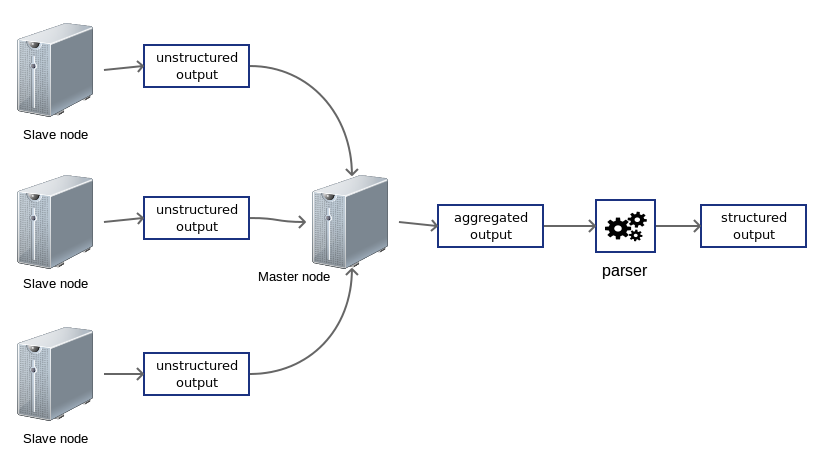
\includegraphics[scale=0.5]{Figures/output_flow.png}
    \rule{25em}{0.5pt}
  \caption[Flow of output through the system]{Flow of output through the system}
  \label{fig:output_flow}
\end{figure}

% ---------

\subsection{Plotting the results}


% --------

% ---------------


\section{Specifying complex test cases}


\begin{enumerate}

\item Create a test file of size 100MB
\item Move it to the mounted shared directory
\item Run IOzone
\item Remove created test files

\end{enumerate}

% --------------


\section{Putting it all together}

\begin{figure}[H]
  \centering
    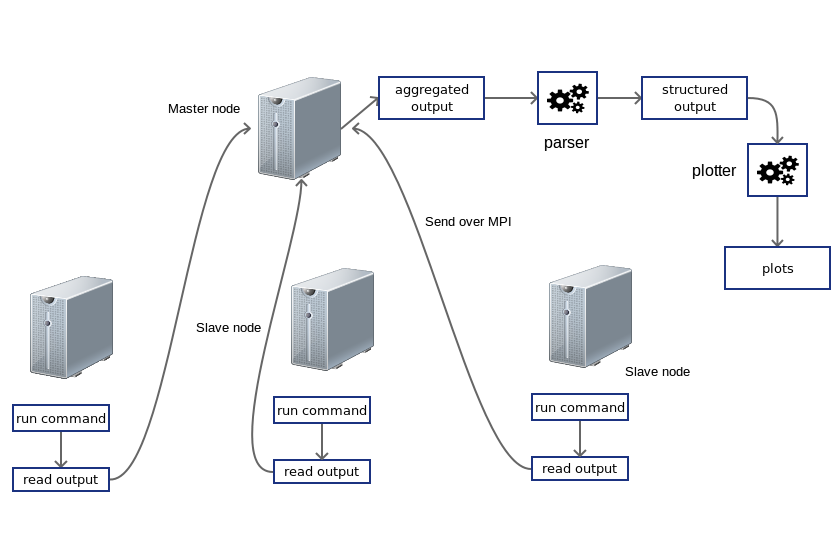
\includegraphics[scale=0.5]{Figures/architecture.png}
    \rule{25em}{0.5pt}
  \caption[General architecture]{General architecture}
  \label{fig:architecture}
\end{figure}


% ------------
